\chapter{Karst and karstification process}
\section{Introduction}
This chapter will briefly describe karst and processes that govern the
development of karts caves.

\section{Basics}

\subsection{Definitions}
\emph{Karstification} is not a strictly defined term. Depending on context it may
mean all forms of corrosion of soluble rocks or it may encompass whole range of
processes that lead to devolopment of karst formations.

Usually karstification means a landscape forming process that consists of dissolution
of various kinds of bedrock. The most common kinds of solutes are limestone,
dolomite, and gypsum \parencite{karstglossary}. However, given right conditions
even some weathering-resistant rocks like quartzite may be subject to 
karstification \parencite{migon2010}\todo{Check reference}.

Although chemical dissolution is the main driving force behind karstification,
mechanical forces may also play a role in the final looks of karst landscape.
That's why sometimes, all these forces together are put under the umbrella term
of karstification.

\emph{Karst} is a terrain formation developed throught means of
\emph{karstification}.

\subsection{Elements of karst landscape}

Karstification process may produce very interesting and varied landscape. Most
common elements of karst landscape will be shown and described.

\begin{figure}
  \centerline{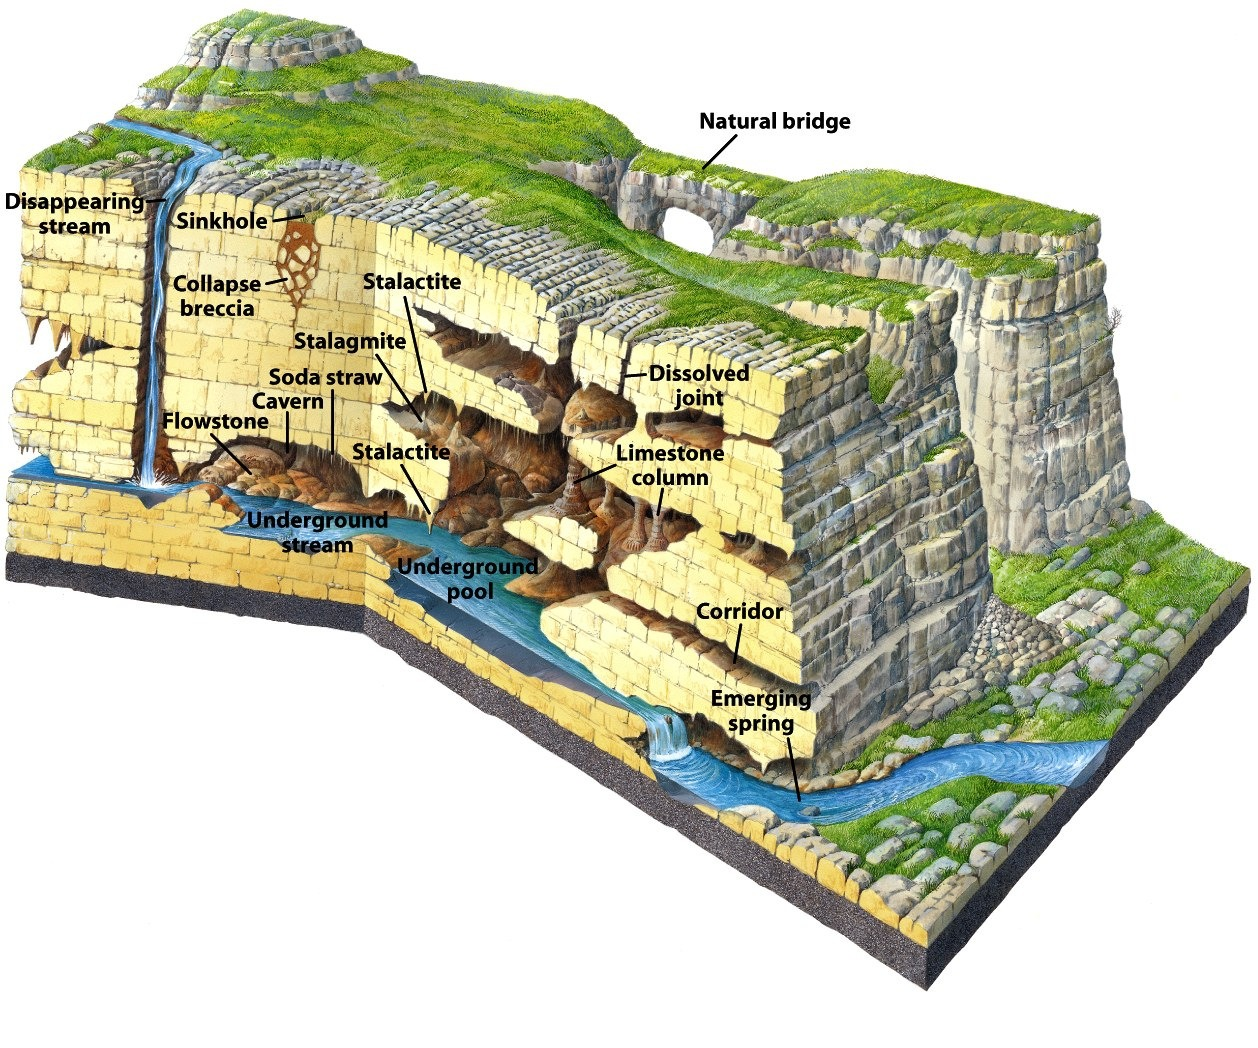
\includegraphics[width=480px]{chapters/karstification/karst_landscape.jpg}}
  \caption{Karst landscape showing various features of karst aquifers.
    Figure from \cite{marshak2006}}
\end{figure}

\section{Overview of karstification process}

Most important factor in karstification process is flow of solvent throught an
underground aquifer. 

\section{Limestone dissolution}

\section{Formation of speleothems}
